\section{LHC Detectors at CERN}
\label{detectors}
There is a vast complex network of different accelerators and different detectors at CERN. The highest energy endpoint in this network is the LHC. The LHC is a \SI{27}{km} counter-rotating accelerator. Using superconducting magnets, it is capable of accelerating protons up to a peak energy level of \SI{7}{TeV}, which results in a peak collision energy of \SI{14}{TeV}. To reach these energy levels, a network of several accelerators is used to initially accelerate the protons to \SI{450}{GeV} before they are injected into the LHC. In the LHC the beams collide with a bunch spacing of \SI{25}{ns} corresponding to a frequency of \SI{40}{MHz} and is called the bunch-crossing (BX) rate. The entire network can be seen in figure \ref{fig:accelerator_network_cern}. More details can be read in the article: LHC Machine \cite{LHCmachine}.

\begin{figure}[H]
    \centering
    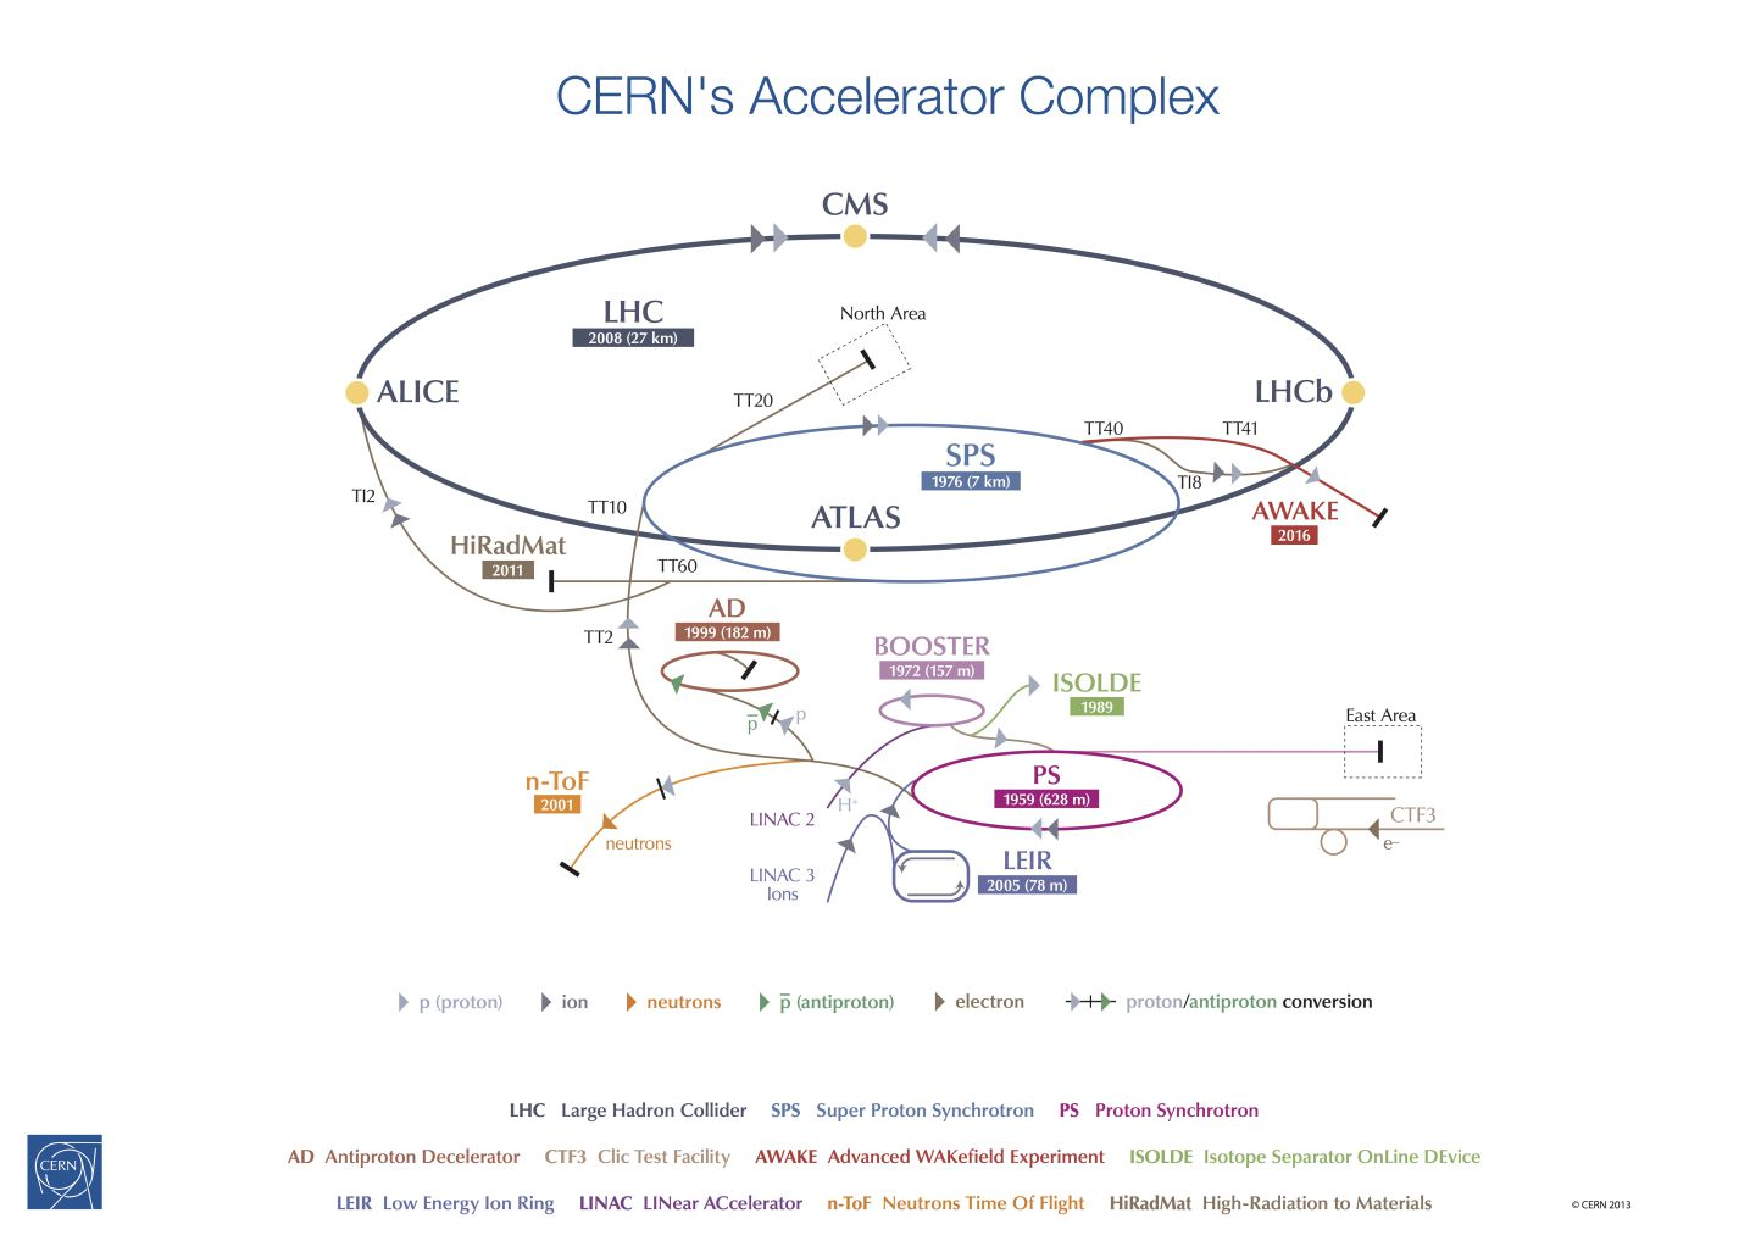
\includegraphics[width=\linewidth]{subfiles/imgs/acceleratorNetworkCERN.pdf}
    \caption{Shows the complete network of used accelerators at CERN (Courtesy of \cite{Haffner:1621894}).}
    \label{fig:accelerator_network_cern}
\end{figure}

There are four detectors placed on the LHC ring. These are A Large Ion Collider Experiment (ALICE), Compact Muon Solenoid (CMS), Large Hadron Collider Beauty (LCHb) and A Toroidal LHC ApparatuS (ATLAS). These 4 experiments can be split into 3 categories. CMS and ATLAS are general-purpose onion detectors, which means they try to detect all particles created by the collision. These two are built in different ways by different independent teams such that they can be used to verify the results of each other. ALICE is an experiment focused on the collision of heavier ions, e.g. lead ions. LCHb is a detector focused on only detecting the particles created by collision, which moves in the beam direction. This makes it possible for them to make a specialized detector better suited for detecting the particles in that specific direction. A majority of the particles created in this experiment are related to the beauty quark, which gives reason to its name. A detailed description of CMS, one of the general-purpose experiments, will now be given. This will lay the foundation for understanding the environment in which the electonics are expected to survie and give a reasoning to some of the design choices made later.

The CMS sits at one of the four collision points in LHC. Figure \ref{fig:cms_layout} shows the layout of the CMS detector. The particles generated in the collisions propagate radially, traversing the silicon tracker. The silicon tracker measures the particle trajectory and transverse momentum $p_T$. The silicon tracker is composed of an all-silicon pixel and strip tracker \cite{collaboration2008cms}. Next are the electromagnetic calorimeter (ECAL) and the hadron calorimeter (HCAL). The calorimeters enable the evaluation of the particle energy. The ECAL uses lead tungstate scintillating crystals for this purpose \cite{collaboration2008cms}. Scintillating crystals emit photons when ionizing particles pass through them. The light is then detected by silicon avalanche photodiodes (APD) in the barrel region and vacuum phototriodes (VPT) in the endcap region. The APD makes use of the avalanche effect, where a single charged particle can knock multiple electrons out of their bond and thereby amplifying their electrical signature. The VPTs are single amplification stage photomultipliers. They have a photocathode at ground potential, a single dynode biased at \SI{+600}{V}, and an anode biased at \SI{+800}{V}. VPTs operate by a photon hitting the cathode which releases electrons. The released photoelectrons are accelerated towards the dynode, where each photoelectron releases multiple new photoelectrons. These are then accelerated towards the anode as it is at a higher potential. The anode then produces an amplified current.     

After the ECAL, the particles enter a brass/scintillator HCAL \cite{collaboration2008cms}. Here the scintillation light is collected by wavelength-shifting (WLS) fibers embedded in the scintillator tiles. The WLS fibers emit multiple low-energy photons for each high-energy photon strike. This light is channeled to photodiodes which amplify the signal. The aforementioned components are encapsulated by a \SI{3.8}{T} superconducting solenoid. Outside the superconducting solenoid, the iron return yoke with muon chambers is placed. The iron return yoke confines the magnetic field and stops all remaining particles except for muons and neutrinos. The muon system has 3 functions: muon identification, momentum measurement, and triggering. In the barrel, region detection is done using drift tubes while in the end-cap region it is done using cathode strip chambers. Both of these systems are completed by a dedicated trigger system of resistive plate chambers.

In total, the CMS detector has a diameter of \SI{15}{m}, a length of \SI{28.7}{m}, and weighs $14 \cdot 10^6$ \si{kg}.

\begin{figure}[H]
    \centering
    \includegraphics[width=\linewidth]{subfiles/imgs/cms_layout.png}
    \caption{Shows the layout of the CMS detector \cite{CMSdetector}.}
    \label{fig:cms_layout}
\end{figure}

The CMS is capable of detecting a wide range of particles using the collection of the data from each of its components. Different particles will follow a different path through the detector based on their charge, momentum, and trajectory. In figure \ref{fig:particles_in_cms} a path of the common particles can be seen. The superconducting solenoid enables the estimation of the charge and momentum of a particle. The charge can be determined by the bend direction of the trajectory because positively charged particles will bend opposite to negatively charged particles and neutral particles will not bend at all. The momentum can then be estimated by the degree of bending as faster-moving particles will bend less than slow-moving particles. 

\begin{figure}[H]
    \centering
    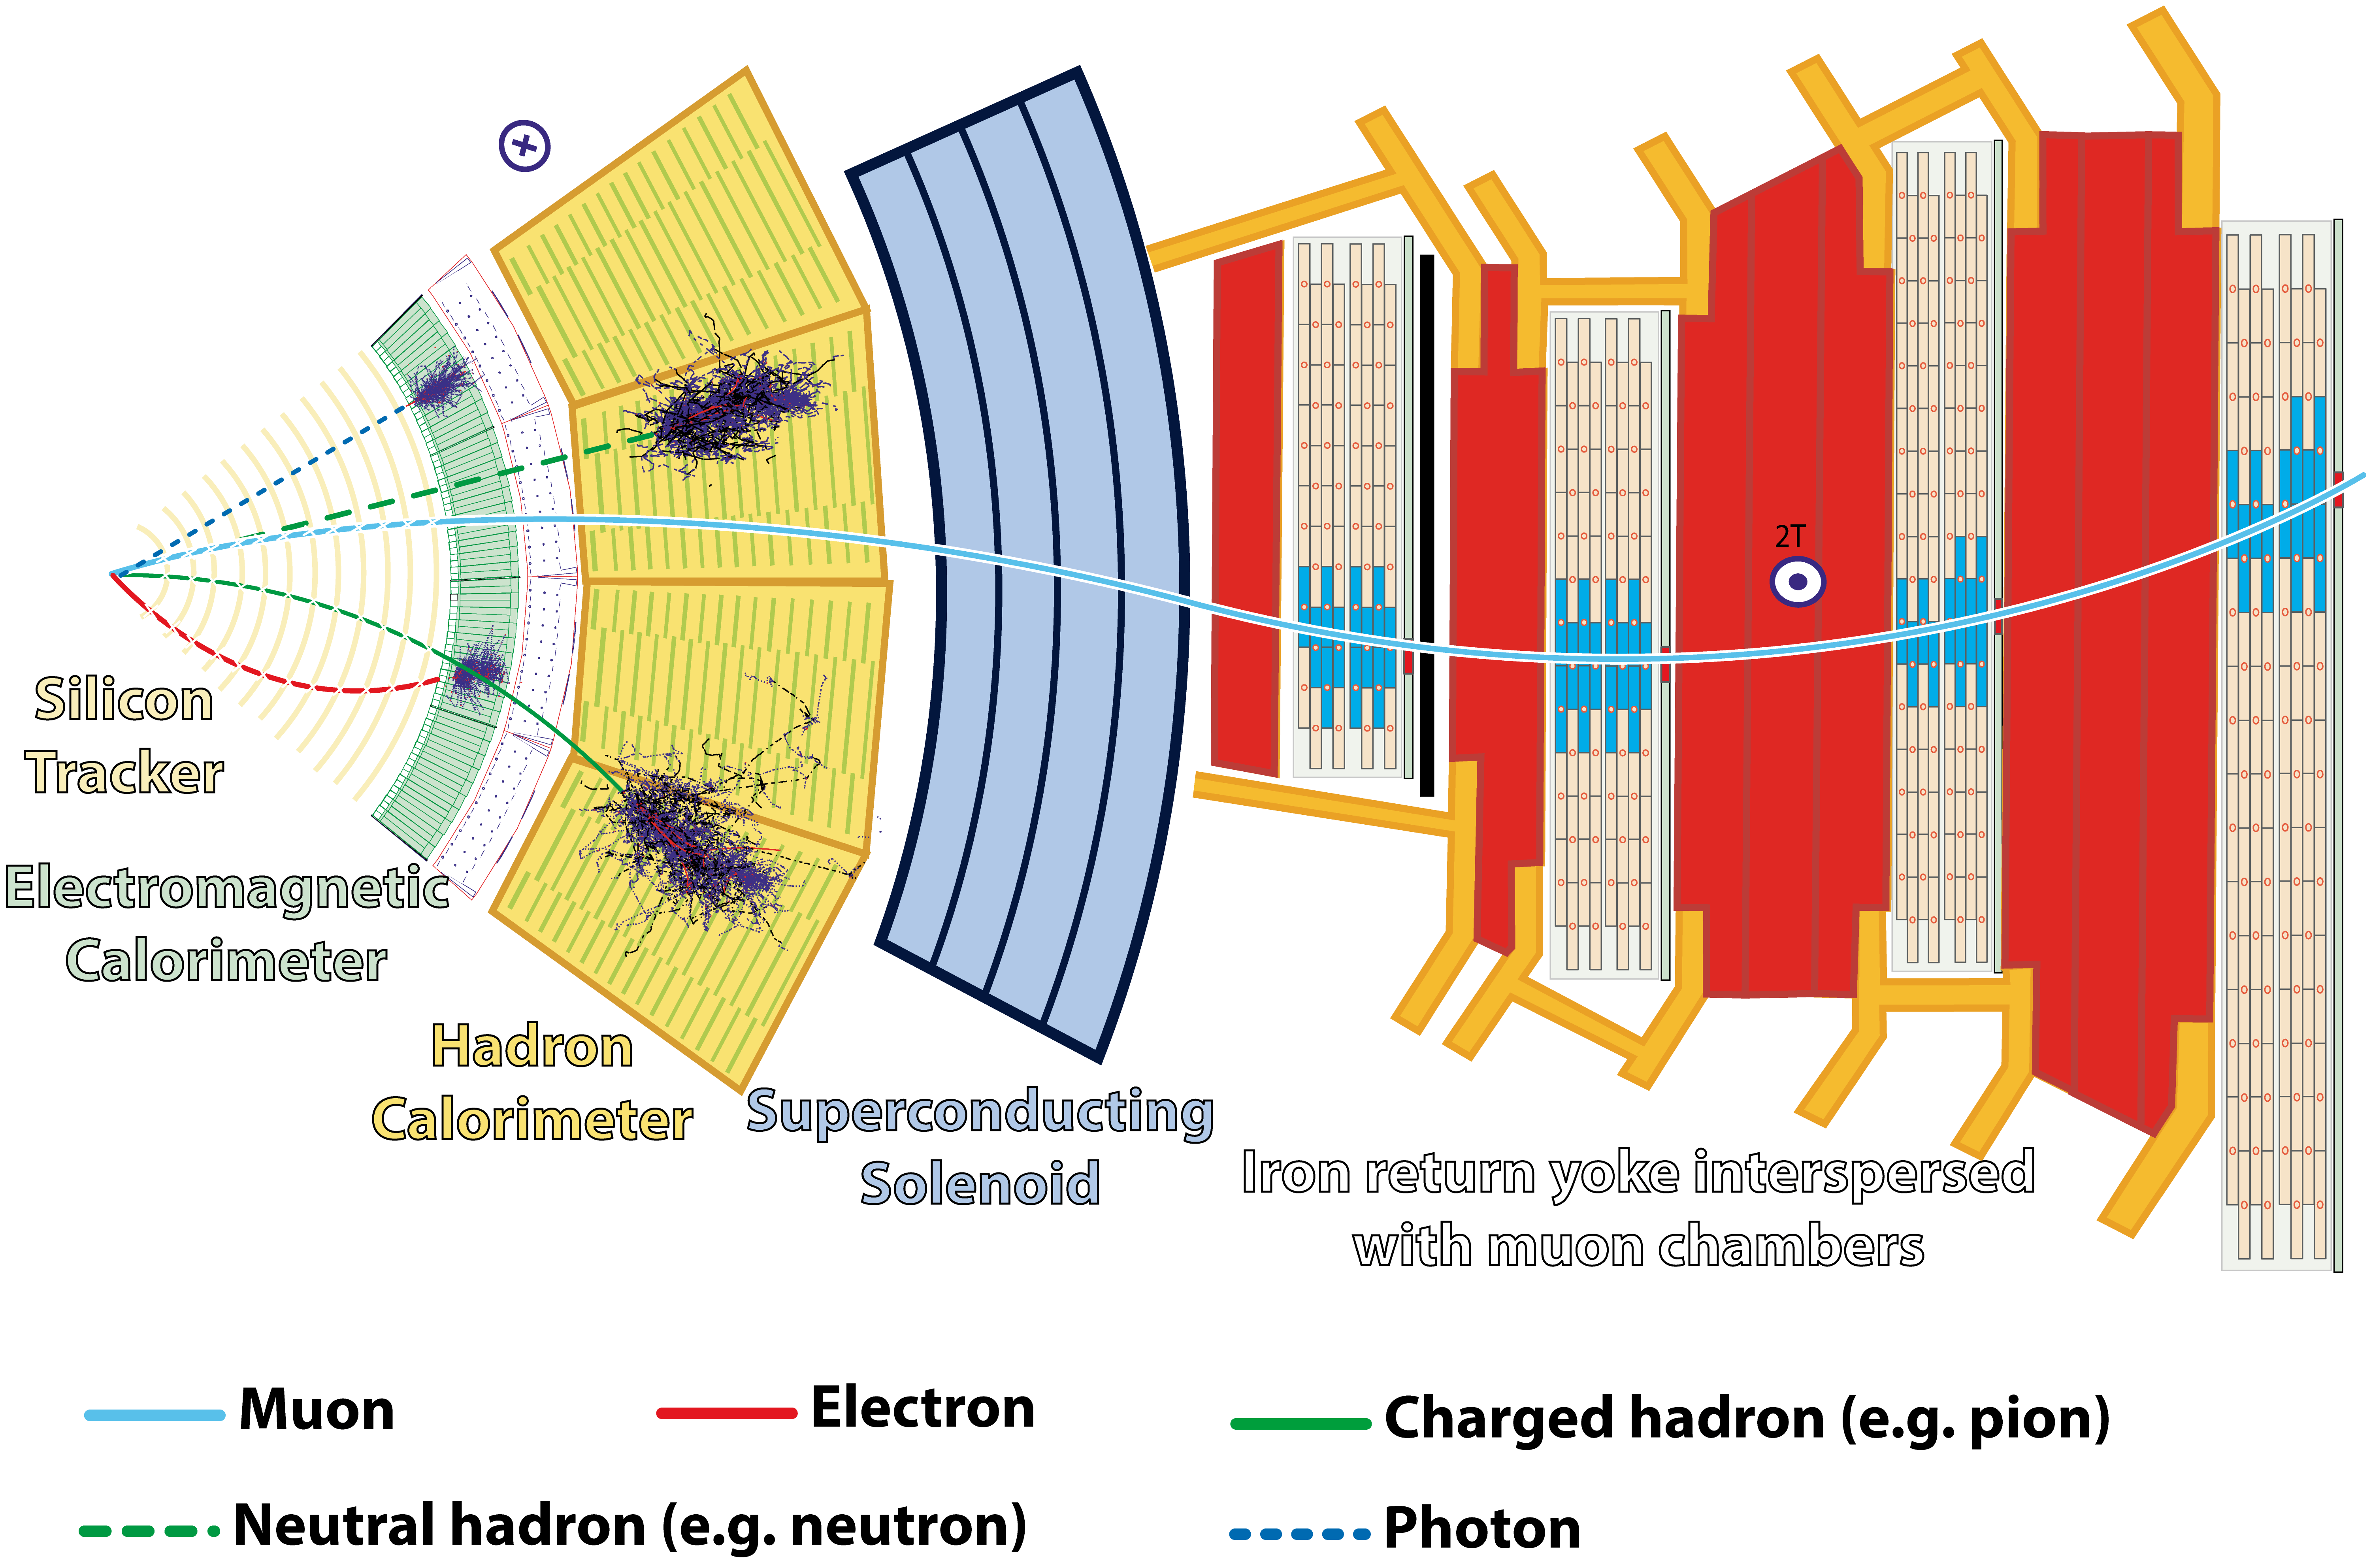
\includegraphics[width=\linewidth]{subfiles/imgs/CMSslice_whiteBackground.png}
    \caption{Shows the movement of different particles in the CMS detector \cite{Barney:2120661}.}
    \label{fig:particles_in_cms}
\end{figure}

The collision of charged particles in the LHC creates ionizing particles which over time will accumulate. The total ionizing dose (TID) expected after 10 years of operation has been simulated using FLUKA, a tool for monte carlo simulation of particle movement and their interactions. The expected dose decreases with distance from the collision point. A complete map of the expected TID for the detector can be seen in figure \ref{fig:tid_in_cms}.  

\begin{figure}[H]
    \centering
    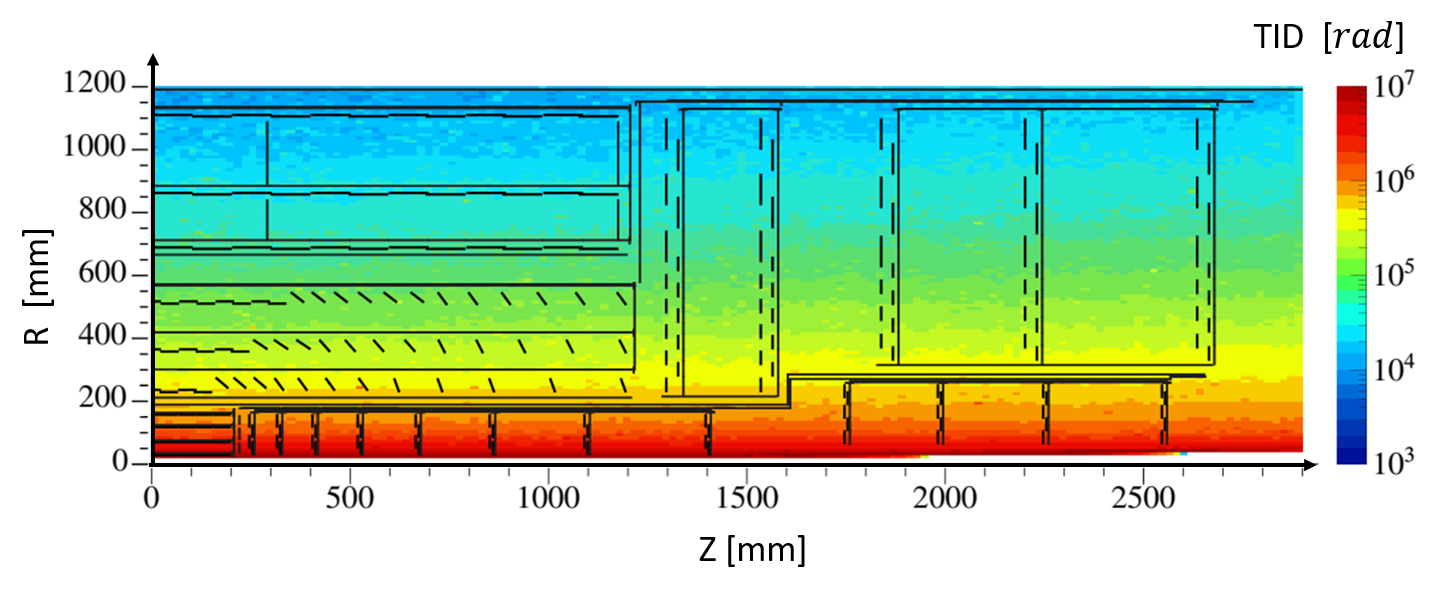
\includegraphics[width=\linewidth]{subfiles/imgs/CMS_RadiationLevels_2.png}
    \caption{Shows expected total ionizing dose in \si{Gy} during a 10-year operation period of the CMS. This is simulated using FLUKA. \cite{cms_tdr}}
    \label{fig:tid_in_cms}
\end{figure}

The ionizing dose and charged particles passing through electronics can alter their behavior and affect the output in unwanted ways. These effects will now be discussed in detail. 
